% !TeX spellcheck = es_ES
\documentclass[titlepage]{article}
\usepackage[utf8]{inputenc}
\usepackage[letterpaper, margin=2.5cm]{geometry}
\usepackage[spanish]{babel}
\usepackage{listings}
\usepackage{float}
\usepackage{graphicx} 
\usepackage{color}
\usepackage[nottoc,notlot,notlof]{tocbibind}
\definecolor{dkgreen}{rgb}{0,0.6,0}
\definecolor{gray}{rgb}{0.5,0.5,0.5}
\definecolor{mauve}{RGB}{253,151,31}
\definecolor{deepred}{RGB}{249,38,114}

\lstset{frame=tb,
    language=Python,
    aboveskip=3mm,
    belowskip=3mm,
    showstringspaces=false,
    columns=flexible,
    numbers=left,
    stepnumber=1,
    basicstyle={\small\ttfamily},
    numberstyle=\tiny\color{gray},
    keywordstyle=\color{blue},
    commentstyle=\color{dkgreen},
    stringstyle=\color{mauve},
    breaklines=true,
    breakatwhitespace=true,
    tabsize=2,
    morekeywords={self, append},
    emph={Transicion, __init__, True, False, __str__, AFN, AFD},
    emphstyle=\color{deepred}
}

\title{Reporte: Práctica 1}
\author{Barrera Pérez Carlos Tonatihu \\ Profesor: Saucedo Delgado Rafael Norman \\ Compiladores \\ Grupo: 3CM6 }

\begin{document}
	\maketitle
	\tableofcontents
	\newpage
	\section{Introducción}
	Los autómatas finitos no determinista y determinista nos permiten identificar si una cadena (secuencia de símbolos) 
	pertenece a un determinado lenguaje regular. Las principales diferencias entre estos dos tipos de autómatas son las siguientes.
	
	\begin{itemize}
		\item \textbf{Autómata finito no determinista}: Un mismo símbolo puede conducir a diferentes estados desde un mismo estado, 
		además, la cadena vacía es valida \cite{compis}.
		\item \textbf{Autómata finito determinista}: El autómata tiene por cada estado y por cada símbolo sólo una transición hacia otro estado \cite{compis}.
	\end{itemize}

	La descripción formal de un autómata determinista $A$ es la siguientes \cite{automata}.
	\[ A = (Q, \Sigma , \delta, q_{0}, F) \]
	Donde:
	
	\begin{itemize}
		\item $Q$ es un conjunto de estados finitos.
		\item $\Sigma$ es un conjunto finito de símbolos de entrada.
		\item $\delta$ es una función de transición que toma como argumentos un estado y un símbolo y retorna un nuevo estado. 
		En un autómata no determinista la función devuelve un conjunto de estados que pertenecen a $Q$.
		\item $q_{0}$ es un estado inicial que pertenece al conjunto de estados finitos $Q$.
		\item $F$ es un conjunto de estados finales que pertenecen al conjunto $Q$.

	\end{itemize}

	\begin{figure}[H]
		\begin{center}
			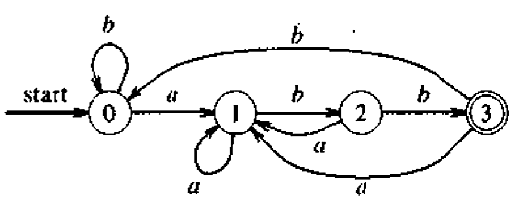
\includegraphics[width=8cm, height=3cm]{AFD.png}
			\caption{Ejemplo de un AFD que reconoce el lenguaje $(a|b)^{*}abb$.}
			\label{fig:AFD}
		\end{center}
	\end{figure}
	Todas estas características fueron importantes en esta práctica ya que al tenerlas en consideración se pudieron 
	modelar los dos tipos de autómatas mediante el uso de programación orientada a objetos en este caso se utilizo Python. 
	Y con ello poder representar cualquier autómata finito a partir de los elementos que lo componen.
	\newpage
	\section{Desarrollo}
	En esta práctica se uso el paradigma orientado a objetos para poder modelar cualquier autómata finito determinista 
	o no determinista con base a sus componentes y con esto poder evaluar cualquier cadena y poder determinar 
	si pertenece a algún determinado lenguaje. Se programaron 3 clases, una para el autómata determinista, otra para el no determinista y una clase extra para poder
	representar las transiciones que se realizan de una manera más fácil
	
	Primero tenemos el código de la clase \emph{Transición}.
	\begin{lstlisting}
	class Transicion:
	  def __init__(self, actual, siguiente, caracter):
	    self.actual = actual
	    self.siguiente = siguiente
	    self.caracter = caracter
	    
	  # Metodo para poder imprimir de forma legible una instancia de esta clase
	  def __str__(self):
	    return '{}->{}: {}'.format(self.actual, self.siguiente, self.caracter)
	\end{lstlisting}
	Como se puede observar en el código nuestra transición consiste de un estado actual, uno siguiente y un símbolo que realiza esa transición.
	Esto nos ayudara a modelar las clases de los autómatas de una manera más clara.
	
	El código de la clase \emph{AFN} fue el siguiente:
	\begin{lstlisting}
	 class AFN:
	 # Usamos la clase set de python para trabajar con los componenetes del automata 
    def __init__(self):
        self.alfabeto = set()
        self.estados_finales = set()
        self.estado_inicial = 0
        self.estados_actuales = list()
        self.transiciones = list()
        self.estados = set()
        self.estado_error = -1

    def agregar_transicion(self, actual, siguiente, caracter):
        self.transiciones.append(Transicion(actual, siguiente, caracter))

    def agregar_finales(self, estados):
        self.estados_finales = estados

    def agregar_alfabeto(self, alfabeto):
        self.alfabeto = alfabeto
        self.alfabeto.add('e')

    def agregar_inicial(self, estado):
        self.estado_inicial = estado

    def agregar_estado(self, estado):
        if estado in self.estados:
            print("Estado repetido")
        else:
            self.estados.add(estado)

    def evaluar_cadena(self, cadena):
        self.estados_actuales = self.estados_epsilon(self.estado_inicial)
        for caracter in cadena:
            if caracter not in self.alfabeto:
                return False
            siguientes_estados = self.obtener_siguientes(caracter)
            self.estados_actuales = []
            for e in siguientes_estados:
                self.estados_actuales.extend(self.estados_epsilon(e))

        for estado in self.estados_actuales:
            if estado in self.estados_finales:
                return True
        return False

    def obtener_siguientes(self, caracter):
        siguientes = list()
        for estado in self.estados_actuales:
            for transicion in self.transiciones:
                if estado == transicion.actual and transicion.caracter == caracter:
                    siguientes.append(transicion.siguiente)
        return siguientes

    def estados_epsilon(self, estados):
        epsilon = list()
        epsilon.append(estados)
        for estado in epsilon:
            for t in self.transiciones:
                if t.caracter == 'e' and t.actual == estado and (t.siguiente not in epsilon):
                    epsilon.append(t.siguiente)
        return epsilon
	\end{lstlisting}
	
	Los métodos principales en esta clase son el que permite obtener los estados épsilon y los estados que se obtienen al evaluar un estado con algún símbolo por lo que al ejecutarlos en conjunto obtenemos un conjunto de nuevos estados "siguientes" por lo que constantemente iremos actualizando los estados en los que nos encontramos, y con esto simular la tabla de transiciones usada para evaluar este tipo de autómatas \cite{compis}.
	
	\begin{figure}[H]
		\begin{center}
			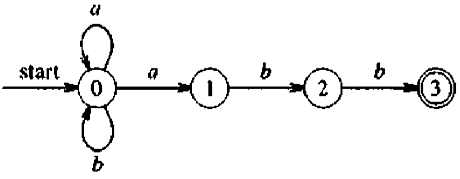
\includegraphics[width=8cm, height=3cm]{AFN.png}
			\caption{AFN que reconoce el lenguaje $(a|b)^{*}abb$.}
			\label{fig:AFN}
		\end{center}
	\end{figure}
	
	El resto de métodos son para establecer los valores iniciales del AFN.
	El código de la clase \emph{AFD} hereda muchas propiedades y métodos de la clase \emph{AFN} modificando el método que se encarga de la evaluación de la cadena.
	
	\begin{lstlisting}
class AFD(AFN):
  def agregar_alfabeto(self, alfabeto):
    self.alfabeto = alfabeto

  def evaluar_cadena(self, cadena):
    self.estados_actuales.append(self.estado_inicial)
    continuar = True
    for caracter in cadena:
      if caracter not in self.alfabeto:
        return False
      for transicion in self.transiciones:
        if transicion.actual == self.estados_actuales[0]:
          if transicion.caracter == caracter:
            self.estados_actuales[0] = transicion.siguiente
            continuar = True
            break
        else:
          continuar = False
      if not continuar:
       self.estados_actuales[0] = self.estado_error

    return self.estados_actuales[0] in self.estados_finales
	\end{lstlisting}
	
	El método es similar al usado en la clase para el autómata no determinista pero sin usar el método que nos permite obtener transiciones épsilon y por ende solo puede hacer un movimiento a la vez por cada estado que tenemos, esto se ve reflejado en la variable \emph{estados\_actuales} la cual solamente tiene un valor a diferencia de tener un conjunto de estados como en el código para el AFN.
	
	\section{Resultados}
	Después de la implementación de estas clases se hicieron pruebas para poder verificar que funcionaran correctamente. Un ejemplo de eso se ve en el siguiente código el cual realiza las pruebas sobre el autómata no determinista de la figura \ref{fig:AFN}.
	
	\begin{lstlisting}
	# Creamos un AFN con todos sus componentes y realizamos 5 pruebas con
	# diferentes cadenas
	
	def correr_automata_AFN():
		print("Automata no determinista")
		automata = AFN()
		automata.agregar_alfabeto({'a', 'b'})
		automata.agregar_estado(0)
		automata.agregar_estado(1)
		automata.agregar_estado(2)
		automata.agregar_estado(3)
		
		automata.agregar_inicial(0)
		automata.agregar_finales({3})
		
		automata.agregar_transicion(0, 1, 'a')
		automata.agregar_transicion(1, 2, 'b')
		automata.agregar_transicion(2, 3, 'b')
		automata.agregar_transicion(0, 0, 'a')
		automata.agregar_transicion(0, 0, 'b')
		
		for n in range(5):
			cadena = input("-Ingresa una cadena: ")
			print("La cadena es:")
			if automata.evaluar_cadena(cadena):
				print("Valida")
			else:
				print("No valida")
	\end{lstlisting}
	
	El resultado fue el siguiente:
	
	\begin{figure}[H]
		\begin{center}
			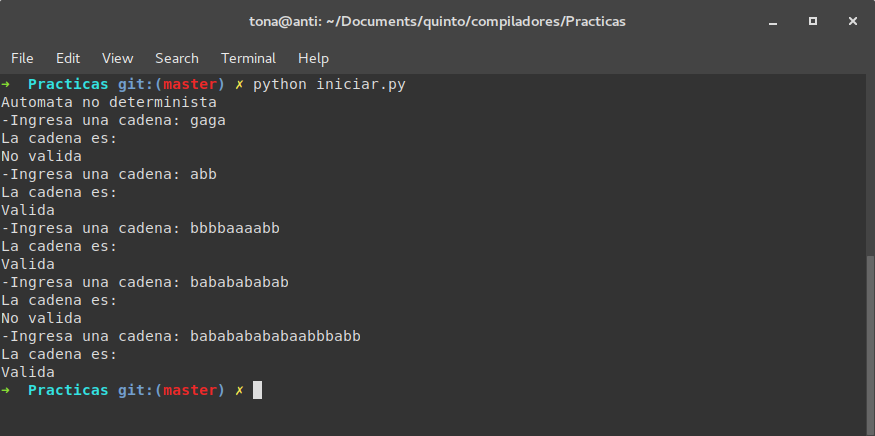
\includegraphics[width=16cm]{AFNprueba.png}
			\caption{Pruebas realizadas sobre el AFN.}
			\label{fig:AFN2}
		\end{center}
	\end{figure}
	
	Por lo que podemos concluir que la clase AFN realiza correctamente su función.
	
	Por otra parte, el autómata determinista de la figura \ref{fig:AFD} fue probado con la siguiente función.
	
	\begin{lstlisting}
	def correr_automata_AFD():
		print("Automata determinista")
		automata = AFD()
		automata.agregar_alfabeto({'a', 'b'})
		automata.agregar_estado(0)
		automata.agregar_estado(1)
		automata.agregar_estado(2)
		automata.agregar_estado(3)
		
		automata.agregar_inicial(0)
		automata.agregar_finales({3})
		
		automata.agregar_transicion(0, 1, 'a')
		automata.agregar_transicion(1, 2, 'b')
		automata.agregar_transicion(2, 3, 'b')
		automata.agregar_transicion(0, 0, 'b')
		automata.agregar_transicion(1, 1, 'a')
		automata.agregar_transicion(2, 1, 'a')
		automata.agregar_transicion(3, 1, 'a')
		automata.agregar_transicion(3, 0, 'b')
		
		for n in range(5):
			cadena = input("-Ingresa una cadena: ")
			print("La cadena es:")
			if automata.evaluar_cadena(cadena):
				print("Valida")
			else:
				print("No valida")
	\end{lstlisting}
	
	El resultado de las pruebas fue el siguiente:
	
	\begin{figure}[H]
		\begin{center}
			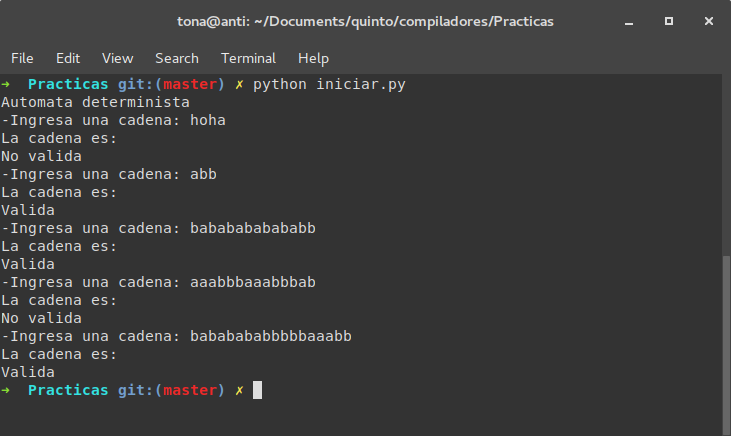
\includegraphics[width=14cm]{AFDprueba.png}
			\caption{Pruebas realizadas sobre el AFD.}
			\label{fig:AFD2}
		\end{center}
	\end{figure}

	De esta forma podemos llegamos a la conclusión de que el autómata funciona de forma correcta.
	
	\section{Conclusiones}
	Fue indispensable conocer los componentes de este tipo de autómatas ademas de saber el como trabajan 
	ya que sin este conocimiento seria imposible el poder modelarlos en una clase. La parte difícil de esta 
	práctica fue el AFN ya que al poder ir a varios estados desde una mismo con el mismo símbolo por lo que 
	aumenta su complejidad al aumentar el numero de caminos que se pueden tomar. 
	Así que el revisar libros y ejercicios relacionados con este tema fue importante para poder solucionar este problema.
	\bibliography{bibliografia} 
	\bibliographystyle{ieeetr}
\end{document}
